\documentclass{article}
\usepackage[utf8]{inputenc}
\usepackage[super,square]{natbib}
\usepackage{tabularx}
\usepackage{parskip}
\usepackage[margin=1.4in]{geometry}
\usepackage{csquotes}
\usepackage{amsmath}
\usepackage{amsfonts}
\usepackage{amsthm}
\usepackage{hyperref}
\usepackage{float}
\usepackage{enumerate}
\usepackage{multicol}
\usepackage{graphicx}
\usepackage{float}

\newcommand{\comment}[1]{}

\title{\vspace{-3cm} Distributed Systems Design and Concepts}
\author{}
\date{}

\comment{
}

\begin{document}
\maketitle
\vspace{-1.5cm}
\tableofcontents
\newpage

\section{Databases}
    \subsection{Data Models and Query Languages}
    Historically, data started out being represented as one big tree (the hierarchical model), but that wasn’t good for representing many-to-many relationships, so the \textbf{relational} SQL datastore model was invented to solve that problem. More recently, developers found that some applications don’t fit well in the relational model either. New nonrelational NoSQL datastores have diverged in two main directions:
    \begin{enumerate}[i.]
        \item \textbf{Document databases} target use cases where data comes in self-contained documents and relationships between one document and another are rare.
        \item \textbf{Graph databases} go in the opposite direction, targeting use cases where anything is potentially related to everything.
    \end{enumerate}
    
    All three models (document, relational, and graph) are widely used today, and each is good in its respective domain. One model can be emulated in terms of another model —for example, graph data can be represented in a relational database—but the result is often awkward. That’s why we have different systems for different purposes, not a single one-size-fits-all solution. 
    
    One thing that document and graph databases have in common is that they typically don’t enforce a schema for the data they store, which can make it easier to adapt applications to changing requirements. However, your application most likely still assumes that data has a certain structure; it’s just a question of whether the schema is explicit (enforced on write) or implicit (handled on read).
    
    Each data model comes with its own query language or framework, i.e. SQL, MapReduce, MongoDB’s aggregation pipeline, Cypher, SPARQL, or Datalog. 
    
    
    \subsection{Storage and Retrieval }
    On a high level, storage engines fall into two broad categories: 
    \begin{enumerate}[i.]
        \item  those optimized for transaction processing (OLTP) and
        \item those optimized for analytics (OLAP).
    \end{enumerate}
    
    There are major differences between the access patterns in those use cases.
    
    \subsubsection{Online Transactional Processing}
    Online Transactional Processing (OLTP) systems are typically user-facing, which means that they may see a huge volume of requests. In order to handle the load, applications usually only touch a small number of records in each query. The application requests records using some kind of key, and the storage engine uses an index to find the data for the requested key. Disk seek time is often the bottleneck here
    
    On the OLTP side, storage engines from two main schools of thought:
    
    \begin{enumerate}[i.]
        \item The \textbf{log-structured} school, which only permits appending to files and deleting obsolete files, but never updates a file that has been written. Bitcask, SSTables, LSM-trees, LevelDB, Cassandra, HBase, Lucene, and others belong to this group.
        
        Log-structured storage engines are a comparatively recent development. Their key idea is that they systematically turn random-access writes into sequential writes on disk, which enables higher write throughput due to the performance characteristics of hard drives and SSDs.
        
        \item The \textbf{update-in-place} school, which treats the disk as a set of fixed-size pages that can be overwritten. \textbf{B-trees} are the biggest example of this philosophy, being used in all major relational databases and also many nonrelational ones.
    \end{enumerate}
    
    \subsubsection{Online Analytical Processing}
    Online Analytical Processing (OLAP) is the technology behind many Business Intelligence (BI) applications. OLAP is a powerful technology for data discovery, including capabilities for limitless report viewing, complex analytical calculations, and predictive “what if” scenario (budget, forecast) planning.

    \textbf{Data warehouses} and similar analytic systems are less well known, because they are primarily used by business analysts, not by end users. They handle a much lower volume of queries than OLTP systems, but each query is typically very demanding, requiring many millions of records to be scanned in a short time. Disk bandwidth (not seek time) is often the bottleneck here, and column-oriented storage is an increasingly popular solution for this kind of workload.
    
    This background illustrated why analytic workloads are so different from OLTP: when your queries require sequentially scanning across a large number of rows, indexes are much less relevant. Instead it becomes important to encode data very compactly, to minimize the amount of data that the query needs to read from disk. Column-oriented storage helps achieve this goal.
    
    \subsection{Concepts}
    \subsubsection{CAP Theorem}
    The CAP theorem (Brewer's theorem) implies that in the presence of a network partition, one has to choose between consistency and availability. It is impossible for a distributed data store to simultaneously provide more than two out of the following three guarantees:
    \begin{enumerate}[i.]
        \item \textbf{Consistency} -- Every read receives the most recent write or an error.
        \item \textbf{Availability} -- Every request receives a (non-error) response, without the guarantee that it contains the most recent write.
        \item \textbf{Partition tolerance} -- The system continues to operate despite an arbitrary number of messages being dropped (or delayed) by the network between nodes.
    \end{enumerate}
    In a distributed system, selecting P (Partition tolerance) is mandatory, that is, you can only choose AP or CP. For example: when a network partition failure happens, should we decide to cancel the operation and thus decrease the availability but ensure consistency, or proceed with the operation and thus provide availability but risk inconsistency.
    
    If a system chooses to provide Consistency over Availability in the presence of partitions and moreover, failures, it will preserve the guarantees of its atomic reads and writes by refusing to respond to some requests. It may decide to shut down entirely (like the clients of a single-node data store), refuse writes (like Two-Phase Commit), or only respond to reads and writes for pieces of data whose ``master” node is inside the partition component (like Membase).
    
    If a system chooses to provide Availability over Consistency in the presence of partitions (i.e. failures), it will respond to all requests, potentially returning stale reads and accepting conflicting writes. These inconsistencies are often resolved via causal ordering mechanisms like vector clocks and application-specific conflict resolution procedures. (Dynamo systems usually offer both of these; Cassandra’s hard-coded Last-Writer-Wins conflict resolution being the main exception.)
    
    CAP theorem is well-suited for critiquing a distributed system design, and understanding what trade-offs need to be made. Taking a system design and iterating through the constraints CAP puts on its subsystems will leave you with a better design at the end. 
    
    \subsubsection{Online analytic processing (OLAP)}
    Online analytic processing (OLAP) is an access pattern characterized by aggregating (e.g., count, sum, average) over a large number of records.

    \subsubsection{Online transaction processing (OLTP)}
    Online transaction processing (OLTP) is an access pattern characterized by fast queries that read or write a small number of records, usually indexed by key
    
    \subsubsection{ACID (SQL)}
    \begin{enumerate}[i.]
        \item \textbf{Atomicity} -- All operations in a transaction succeed or every operation is rolled back.
        \item \textbf{Consistency} -- On the completion of a transaction, the database is structurally sound.
        \item \textbf{Isolation} -- Transactions do not contend with one another. Contentious access to data is moderated by the database so that transactions appear to run sequentially.
        \item \textbf{Durability} -- The results of applying a transaction are permanent, even in the presence of failures.
    \end{enumerate}
    
    \subsubsection{Primary and Foreign Keys}
    A primary key is a value (typically a number or a string) that uniquely identifies a record. In many applications, primary keys are generated by the system when a record is created (e.g., sequentially or randomly); they are not usually set by users.
    
    A foreign key is a column or group of columns in a relational database table that provides a link between data in two tables. It acts as a cross-reference between tables because it references the primary key of another table, thereby establishing a link between them
    
    The more ids required to get to a piece of data, the more options you have in partitioning the data. The fewer ids required to get a piece of data, the easier it is to consume your system’s output.
    
    Watch out for what kind of information you encode in your ids, explicitly and implicitly. Clients may use the structure of your ids to de-anonymize private data, crawl your system in unexpected ways (auto-incrementing ids are a typical sore point), or perform a host of other attacks.
    
    
    \subsubsection{Normalized Data}
    Normalized Data is structured in such a way that there is no redundancy or duplication. In a normalized database, when some piece of data changes, you only need to change it in one place, not many copies in many different places.
    
    \subsubsection{Derived Data, Joins, Materialized Views}
    A derived dataset is created from some other data through a repeatable process, which you could run again if necessary. Usually, derived data is needed to speed up a particular kind of read access to the data.  Indexes, caches, and materialized views are examples of derived data.
    
    A join brings together records that have something in common. Most commonly used in the case where one record has a reference to another (a foreign key, a document reference, an edge in a graph) and a query needs to get the record that the reference points to.
    
    To materialize means to perform a computation preemptively and write out its result, as opposed to calculating it on demand when requested.
    
    \subsubsection{Index and Secondary Index}
    Indexing is a way to get an unordered table into an order that will maximize the query’s efficiency while searching. An index creates a data structure, typically a B-tree, with values from a specific column. It may then use a search algorithm, typically binary search, to find the value and return a pointer to its true index in the unordered table.
    
    A secondary index is an additional data structure that is maintained alongside the primary data storage and which allows you to efficiently search for records that match a certain kind of condition.
    
    \subsubsection{BASE (NoSQL)}
    \begin{enumerate}[i.]
        \item \textbf{Basic availability} -- The database appears to work most of the time.
        \item \textbf{Soft-state} -- Stores don’t have to be write-consistent, nor do different replicas have to be mutually consistent all the time.
        \item \textbf{Eventual consistency} -- Stores exhibit consistency at some later point (e.g., lazily at read time).
    \end{enumerate}
    
    \subsubsection{Types of NoSQL}
    \begin{itemize}
        \item \textbf{Key-value} -- an in-memory hashtable 
        \item \textbf{Wide column} -- names and format of the columns can vary from row to row in the same table. ex: Cassandra. 
        \item \textbf{Document Based} --  relies on internal structure in the document in order to extract metadata for further optimization ex: ElasticSearch
        \item \textbf{Graph Based} -- uses graph structures for semantic queries with nodes, edges, and properties to represent and store data. ex: Neo4j
    \end{itemize}
    
    \subsubsection{Denormalized Data}
    A denormalized dataset introduces some amount of redundancy or duplication in a normalized dataset, typically in the form of a cache or index, in order to speed up reads. A  denormalized value is a kind of precomputed query result, similar to a materialized view.
    
    \subsubsection{Row Store vs. Column Store}
    A \textbf{row store} (or row-oriented database) stores a sequence of records that contains the fields of one row in the table. In a \textbf{column store}, the entries of a column are stored in contiguous memory locations. At a basic level, row stores are great for transaction processing. Column stores are great for highly analytical query models. Row stores have the ability to write data very quickly, whereas a column store excel at aggregating large volumes of data for a subset of columns. By storing data in columns rather than rows, the database can more precisely access the data it needs to answer a query rather than scanning and discarding unwanted data in rows.
    
    Column stores typically make use of Log-structured merge-tree (LSM-Trees) which provide indexed access to files with high insert volume. Row stores typically use B-Trees. Column-compression is a column-level operation that reduces the size of data when it is stored. Compression conserves storage space and reduces the size of data that is read from storage, which reduces the amount of disk I/O and therefore improves query performance.
    
    \subsubsection{Data Warehouse}
    A database in which data from several different OLTP systems has been combined and prepared to be used for analytics purposes, i.e. as an OLAP.
    
    \subsubsection{Extract–Transform–Load}
    Extract–Transform–Load (ETL) is the process of extracting data from a source database, transforming it into a form that is more suitable for analytic queries, and loading it into a data warehouse or batch processing system.
    
    \subsubsection{Stored Procedure}
    A way of encoding the logic of a transaction such that it can be entirely executed  on a database server, without communicating back and forth with a client during the transaction.

\newpage
\section{Concurrency}
    \subsection{Transactions}
    Transactions are an abstraction layer that allows an application to pretend that certain concurrency problems and certain kinds of hardware and software faults don’t exist. A large class of errors is reduced down to a simple transaction abort, and the application just needs to try again.
    
    Not all applications are susceptible to all those problems: an application with very simple access patterns, such as reading and writing only a single record, can probably manage without transactions. However, for more complex access patterns, transactions can hugely reduce the number of potential error cases you need to think about.
    
    Without transactions, various error scenarios (processes crashing, network interruptions, power outages, disk full, unexpected concurrency, etc.) mean that data can become inconsistent in various ways. For example, denormalized data can easily go out of sync with the source data. Without transactions, it becomes very difficult to reason about the effects that complex interacting accesses can have on the database.
    
    In concurrency control there are several widely used isolation levels, in particular read committed, snapshot isolation (sometimes called repeatable read), and serializable. We can characterize those isolation levels through various examples of race conditions:
    
    \begin{enumerate}[i.]
        \item \textbf{Dirty reads} -- One client reads another client’s writes before they have been committed. The read committed isolation level and stronger levels prevent dirty reads.
        
        \item \textbf{Dirty writes} -- One client overwrites data that another client has written, but not yet committed. Almost all transaction implementations prevent dirty writes.
        
        \item \textbf{Read skew (nonrepeatable reads)} -- A client sees different parts of the database at different points in time. This issue is most commonly prevented with snapshot isolation, which allows a transaction   to read from a consistent snapshot at one point in time. It is usually implemented with multi-version concurrency control (MVCC).
        
        \item \textbf{Lost updates} -- Two clients concurrently perform a read-modify-write cycle. One overwrites the other’s write without incorporating its changes, so data is lost. Some implementations of snapshot isolation prevent this anomaly automatically, while others require a manual lock (SELECT FOR UPDATE).
        
        \item \textbf{Write skew} -- A transaction reads something, makes a decision based on the value it saw, and writes the decision to the database. However, by the time the write is made, the premise of the decision is no longer true. Only serializable isolation prevents this  anomaly.
        
        \item \textbf{Phantom reads} -- A transaction reads objects that match some search condition. Another client makes a write that affects the results of that search. Snapshot isolation prevents straightforward phantom reads, but phantoms in the context of write skew require special treatment, such as index-range locks.
    \end{enumerate}
    
    Weak isolation levels protect against some of those anomalies but leave you, the application developer, to handle others manually (e.g., using explicit locking). Only serializable isolation protects against all of these issues. There are three different approaches to implementing serializable transactions:
    
    \begin{enumerate}[i.]
        \item Literally executing transactions in a serial order -- If you can make each transaction very fast to execute, and the transaction throughput is low enough to process on a single CPU core, this is a simple and effective option.
        
        \item  Two-phase locking (2PL) --  For decades this has been the standard way of implementing serializability, but  many applications avoid using it because of its performance characteristics.
        
        \item Serializable snapshot isolation (SSI) -- A fairly new algorithm that avoids most of the downsides of the previous approaches. It uses an optimistic approach, allowing transactions to proceed without blocking. When a transaction wants to commit, it is checked, and it is aborted if the execution was not serializable.
        
    \end{enumerate}
    
    Transactions are a valuable database feature, no matter which data model is used. Transactions in distributed databases open a new set of difficult challenges.
    
    \subsection{Concepts}
    \subsubsection{Concurrency}
    Concurrency is the ability of different parts or units of a program, algorithm, or problem to be executed out-of-order or in partial order, without affecting the final outcome.
    
    \subsubsection{Transactions}
    A transaction groups together several reads and writes into a logical unit, in order to simplify error handling and concurrency issues.
    
    \subsubsection{Multi-Processing and Multi-Threading}
    Multithreading is the ability of a central processing unit (CPU) (or a single core in a multi-core processor) to provide multiple threads of execution concurrently, supported by the operating system.
    
    Where multiprocessing systems include multiple complete processing units in one or more cores, multithreading aims to increase utilization of a single core by using thread-level parallelism, as well as instruction-level parallelism.
    
    \subsubsection{Locks/Mutex}
    A lock  or mutex (from mutual exclusion) is mechanism to ensure that only one thread, node, or transaction can access something, and anyone else who wants to access the same thing must wait until the lock is released. A lock is useful in an environment where there are many threads of execution.
    
    \subsubsection{Deadlocks}
    A deadlock is a state in which each member of a group is waiting for another member, including itself, to take action, such as sending a message or more commonly releasing a lock.

    \subsubsection{Optimistic and Pessimistic Locking}
    Optimistic Locking is a strategy where you read a record, take note of a version number, date, timestamps or checksums/hashes and verify that the version hasn't changed before writing the record back. If the record is dirty (i.e. a different version than yours) you abort the transaction and the user can re-start it. This strategy is most applicable to high-volume systems and three-tier architectures where you do not necessarily maintain a connection to the database for your session.
    
    Pessimistic Locking is where you lock the record for your exclusive use until you have finished with it. It has much better integrity than optimistic locking but requires you to be careful with your application design to avoid deadlocks. To use pessimistic locking you need either a direct connection to the database (as would typically be the case in a two tier client server application) or an externally available transaction ID that can be used independently of the connection.

    \subsubsection{Operational transformation}
    Operational transformation (OT) is a technology for supporting a range of collaboration functionalities in advanced collaborative software systems. OT was originally invented for consistency maintenance and concurrency control in collaborative editing of plain text documents. Its capabilities have been extended and its applications expanded to include group undo, locking, conflict resolution, operation notification and compression, group-awareness, HTML/XML and tree-structured document editing, collaborative office productivity tools, application-sharing, and collaborative computer-aided media design tools.
    
    \subsubsection{Commit log}
    A commit log is a record of transactions. It's used to keep track of what's happening, and help with disaster recovery. Generally, all commits are written to the log before being applied, so transactions that were in flight when the server went down can be recovered and re-applied by checking the log. So when we want to update an entry in machine A, it will first store this request in commit log. And then a separate program will process all the commit logs in order (in a queue). Whenever an operation fails, we can easily recover as we can lookup the commit log.


    \subsubsection{Idempotent}
    Describing an operation that can be safely retried; if it is executed more than once, it has the same effect as if it was only executed once.
    
    \subsubsection{Atomic}
    In the context of concurrent operations: describing an operation that appears to take effect at a single point in time, so another concurrent process can never encounter the operation in a ``half-finished” state.
    
    In the context of transactions: grouping together a set of writes that must either all be committed or all be rolled back, even if faults occur.
    
    \subsubsection{Linearizable}
    Behaving as if there was only a single copy of data in the system, which is updated by atomic operations.
    
    \subsubsection{Serializable}
    A guarantee that if several transactions execute concurrently, they behave the same as if they had executed one at a time, in some serial order.
    
    
    \subsubsection{Isolation}
    In the context of transactions, describing the degree to which concurrently executing transactions can interfere with each other. Serializable isolation provides the strongest guarantees, but weaker isolation levels are also used.
    
    Snapshot isolation is a guarantee that all reads made in a transaction will see a consistent snapshot of the database, and the transaction itself will successfully commit only if no updates it has made conflict with any concurrent updates made since that snapshot.
    
    \subsubsection{Synchronization}
    Process synchronization refers to the idea that multiple processes are to join up or handshake at a certain point, in order to reach an agreement or commit to a certain sequence of action. Data synchronization refers to the idea of keeping multiple copies of a dataset in coherence with one another, or to maintain data integrity.
    
    \subsubsection{CAS}
    Compare-and-swap (CAS) is an atomic instruction used in multithreading to achieve synchronization. It compares the contents of a memory location with a given value and, only if they are the same, modifies the contents of that memory location to a new given value.
    
    \subsubsection{Two-phase locking (2PL)}
    An algorithm for achieving serializable isolation that works by a transaction acquiring a lock on all data it reads or writes, and holding the lock until the end of the transaction.
    
    \subsubsection{Two-phase commit (2PC)}
    An algorithm to ensure that several database nodes either all commit or all abort a transaction.
    
    \subsubsection{Total order}
    A way of comparing things (e.g., time-stamps) that allows you to always say which one of two things is greater and which one is lesser. An ordering in which some things are incomparable (you cannot say which is greater or smaller) is called a partial order.
    
    \subsubsection{Lamport Timestamps and Vector Clock}
    The \textbf{Lamport timestamp} algorithm is a simple logical clock algorithm used to determine the order of events in a distributed computer system. Conceptually, this logical clock can be thought of as a clock that only has meaning in relation to messages moving between processes. When a process receives a message, it re-synchronizes its logical clock with that sender.
    
    A \textbf{vector clock} extends on Lamport timestamps and is used for generating a partial ordering of events in a distributed system and detecting causality violations. 
    
    \begin{itemize}
        \item Initially all clocks are zero.
        
        \item  Each time a process experiences an internal event, it increments its own logical clock in the vector by one.
        
        \item Each time a process sends a message, it increments its own logical clock in the vector by one (but not twice for the same event) and then sends a copy of its own vector.
        
        \item Each time a process receives a message, it increments its own logical clock in the vector by one and updates each element in its vector by taking the maximum of the value in its own vector clock and the value in the vector in the received message (for every element).
    \end{itemize}
    
    \subsubsection{Skew}
    A timing anomaly that causes events to appear in an unexpected, nonsequential order.

\newpage    
\section{Distributed Computing}
    \subsection{Replication}
    Replication can serve several purposes:
    \begin{enumerate}[i.]
        \item \textbf{High availability} --  Keeping the system running, even when one machine (or several machines, or an  entire datacenter) goes down
        
        \item \textbf{Disconnected operation} -- Allowing an application to continue working when there is a network interruption
        
        \item \textbf{Latency} -- Placing data geographically close to users, so that users can interact with it faster

        \item \textbf{Scalability} -- Being able to handle a higher volume of reads than a single machine could handle, by performing reads on replicas
    \end{enumerate}
        
    Despite being a simple goal—keeping a copy of the same data on several machines -- replication turns out to be a remarkably tricky problem. It requires carefully thinking about concurrency and about all the things that can go wrong, and dealing with the consequences of those faults. At a minimum, we need to deal with unavailable nodes and network interruptions (and that’s not even considering the more insidious kinds of fault, such as silent data corruption due to software bugs).
        
    Three main approaches to replication:
    \begin{enumerate}[i.]
        \item \textbf{Single-leader replication} -- Clients send all writes to a single node (the leader), which sends a stream of data change events to the other replicas (followers). Reads can be performed on any replica, but reads from followers might be stale.
        
        \item \textbf{Multi-leader replication} -- Clients send each write to one of several leader nodes, any of which can accept writes. The leaders send streams of data change events to each other and to any follower nodes.
        
        \item \textbf{Leaderless replication} -- Clients send each write to several nodes, and read from several nodes in parallel in order to detect and correct nodes with stale data.
    \end{enumerate}
    
    Each approach has advantages and disadvantages. Single-leader replication is popular because it is fairly easy to understand and there is no conflict resolution to worry about. Multi-leader and leaderless replication can be more robust in the presence of faulty nodes, network interruptions, and latency spikes—at the cost of being harder to reason about and providing only very weak consistency guarantees.
    
    Replication can be synchronous or asynchronous, which has a profound effect on the system behavior when there is a fault. Although asynchronous replication can be fast when the system is running smoothly, it’s important to figure out what happens when replication lag increases and servers fail. If a leader fails and you promote an asynchronously updated follower to be the new leader, recently committed data may be lost.
    
    Some strange effects that can be caused by \textbf{replication lag}, though there exist a few consistency models which are helpful for deciding how an application should behave under replication lag:
    
    \begin{enumerate}[i.]
        \item \textbf{Read-after-write consistency} -- Users should always see data that they submitted themselves
        \item \textbf{Monotonic reads} --  After users have seen the data at one point in time, they shouldn’t later see the data from some earlier point in time
    \end{enumerate}
    
    There are concurrency issues that are inherent in multi-leader and leaderless replication approaches. Because they allow multiple writes to happen concurrently, conflicts may occur.
    
    % TODO: Add details/examples
    There exists algorithms that a database might use to determine whether one operation happened before another, or whether they happened concurrently. There also exist methods for resolving conflicts by merging together concurrent updates
    
    The counterpart of replication is splitting a large data-set into partitions.
    
    \subsection{Partitioning Data}
    Partitioning is necessary when you have so much data that storing and processing it on a single machine is no longer feasible.
    
    The goal of partitioning is to spread the data and query load evenly across multiple machines, avoiding hot spots (nodes with disproportionately high load). This requires choosing a partitioning scheme that is appropriate to your data, and rebalancing the partitions when nodes are added to or removed from the cluster
    
    Two main approaches to partitioning:
    \begin{enumerate}[i.]
        \item \textbf{Key range partitioning} -- where keys are sorted, and a partition owns all the keys from some minimum up to some maximum. Sorting has the advantage that efficient range queries are possible, but there is a risk of hot spots if the application often accesses keys that are close together in the sorted order
        
        In this approach, partitions are typically rebalanced dynamically by splitting the range into two subranges when a partition gets too big
        
        \item \textbf{Hash partitioning} -- where a hash function is applied to each key, and a partition owns a range of hashes. This method destroys the ordering of keys, making range queries inefficient, but may distribute load more evenly. 
        
        When partitioning by hash, it is common to create a fixed number of partitions in advance, to assign several partitions to each node, and to move entire partitions from one node to another when nodes are added or removed. Dynamic partitioning can also be used.
    \end{enumerate}
    
    Hybrid approaches are also possible, for example with a compound key: using one part of the key to identify the partition and another part for the sort order.

    A secondary index also needs to be partitioned, and there are two methods:
    
    \begin{enumerate}[i.]
        \item \textbf{Document-partitioned indexes (local indexes)} --  where the secondary indexes are stored in the same partition as the primary key and value. This means that only a  single partition needs to be updated on write, but a read of the secondary index requires a scatter/gather across all partitions.
        
        \item \textbf{Term-partitioned indexes (global indexes)} -- where the secondary indexes are partitioned separately, using the indexed values. An entry in the secondary index may include records from all partitions of the primary key. When a document is written, several partitions of the secondary index need to be updated; however, a read can be served from a single partition.
    \end{enumerate}

    Techniques for routing queries to the appropriate partition, which range from simple partition-aware load balancing to sophisticated parallel query execution engines.
    
    By design, every partition operates mostly independently—that’s what allows a partitioned database to scale to multiple machines. However, operations that need to write to several partitions can be difficult to reason about: for example, what happens if the write to one partition succeeds, but another fails? 

    \subsection{Fault Tolerance }
    
    \vspace{8pt}
    \[
        P(\text{any failure}) = 1- P(\text{individual node not failing})^{\text{number of nodes} } 
    \]
    
    If you can avoid opening Pandora’s box and simply keep things on a single machine, it is generally worth doing so. There are a wide range of problems that can occur in distributed systems, including:
    
    \begin{enumerate}[i.]
        \item Whenever you try to send a packet over the network, it may be lost or arbitrarily   delayed. Likewise, the reply may be lost or delayed, so if you don’t get a reply, you have no idea whether the message got through.
        \item A node’s clock may be significantly out of sync with other nodes (despite your   best efforts to set up NTP), it may suddenly jump forward or back in time, and relying on it is dangerous because you most likely don’t have a good measure of your clock’s error interval.
        \item A process may pause for a substantial amount of time at any point in its execution (perhaps due to a stop-the-world garbage collector), be declared dead by other nodes, and then come back to life again without realizing that it was paused.
    \end{enumerate}

    The fact that such partial failures can occur is the defining characteristic of distributed systems. Whenever software tries to do anything involving other nodes, there is the possibility that it may occasionally fail, or randomly go slow, or not respond at all (and eventually time out). In distributed systems, we try to build tolerance of partial failures into software, so that the system as a whole may continue functioning even when some of its constituent parts are broken.
    
    To tolerate faults, the first step is to detect them, but even that is hard. Most systems don’t have an accurate mechanism of detecting whether a node has failed, so most distributed algorithms rely on timeouts to determine whether a remote node is still available. However, timeouts can’t distinguish between network and node failures, and variable network delay sometimes causes a node to be falsely suspected of crashing. Moreover, sometimes a node can be in a degraded state: for example, a Gigabit network interface could suddenly drop to 1 Kb/s throughput due to a driver bug. Such a node that is ``limping” but not dead can be even more difficult to deal with than a cleanly failed node.
    
    Once a fault is detected, making a system tolerate it is not easy either: there is no global variable, no shared memory, no common knowledge or any other kind of shared state between the machines. Nodes can’t even agree on what time it is, let alone on anything more profound. The only way information can flow from one node to another is by sending it over the unreliable network. Major decisions cannot be safely made by a single node, so we require protocols that enlist help from other nodes and try to get a quorum to agree.
    
    Scalability is not the only reason for wanting to use a distributed system. Fault tolerance and low latency (by placing data geographically close to users) are equally important goals, and those things cannot be achieved with a single node.
    
    It is possible to give hard real-time response guarantees and bounded delays in networks, but doing so is very expensive and results in lower utilization of hardware resources. Most non-safety-critical systems choose cheap and unreliable over expensive and reliable.
    
    \subsection{Consistency and Consensus }
    \textbf{Linearizability} is a popular consistency model: its goal is to make replicated data appear as though there were only a single copy, and to make all operations act on it atomically. Although linearizability is appealing because it is easy to understand -- it makes a database behave like a variable in a single-threaded program -- it has the downside of being slow, especially in environments with large network delays.
    
    \textbf{Causality} imposes an ordering on events in a system (what happened before what, based on cause and effect). Unlike linearizability, which puts all operations in a single, totally ordered timeline, causality provides us with a weaker consistency model: some things can be concurrent, so the version history is like a timeline with branching and merging. Causal consistency does not have the coordination overhead of linearizability and is much less sensitive to network problems.
    
    However, even if we capture the causal ordering (for example using Lamport time-stamps), some things cannot be implemented this way: for example, in ensuring that a username is unique and rejecting concurrent registrations for the same username. If one node is going to accept a registration, it needs to somehow know that another node isn’t concurrently in the process of registering the same name. This problem led us toward consensus.
    
    Achieving \textbf{consensus} means deciding something in such a way that all nodes agree on what was decided, and such that the decision is irrevocable. With some digging, it turns out that a wide range of problems are actually reducible to consensus and are equivalent to each other (in the sense that if you have a solution for one of them, you can easily transform it into a solution for one of the others). Such equivalent problems include:
    
    \begin{enumerate}[i.]
        \item \textbf{Linearizable compare-and-set registers} -- The register needs to atomically decide whether to set its value, based on whether its current value equals the parameter given in the operation.
        
        \item \textbf{Atomic transaction commit} -- A database must decide whether to commit or abort a distributed transaction.
        
        \item \textbf{Total order broadcast} -- The messaging system must decide on the order in which to deliver messages.
        
        \item \textbf{Locks and leases} --  When several clients are racing to grab a lock or lease, the lock decides which one successfully acquired it.
        
        \item \textbf{Membership/coordination service} -- Given a failure detector (e.g., timeouts), the system must decide which nodes are alive, and which should be considered dead because their sessions timed out.
        
        \item \textbf{Uniqueness constraint} -- When several transactions concurrently try to create conflicting records with the same key, the constraint must decide which one to allow and which should fail with a constraint violation
    \end{enumerate}

    All of these are straightforward if you only have a single node, or if you are willing to assign the decision-making capability to a single node. This is what happens in a \textbf{single-leader database}: all the power to make decisions is vested in the leader, which is why such databases are able to provide linearizable operations, uniqueness constraints, a totally ordered replication log, and more.
    
    However, if that single leader fails, or if a network interruption makes the leader unreachable, such a system becomes unable to make any progress. There are three ways of handling that situation:
    
    \begin{enumerate}[i.]
        \item Wait for the leader to recover, and accept that the system will be blocked in the meantime. Many XA/JTA transaction coordinators choose this option. This approach does not fully solve consensus because it does not satisfy the termination property: if the leader does not recover, the system can be blocked forever.
        
        \item Manually fail over by getting humans to choose a new leader node and reconfigure the system to use it. Many relational databases take this approach. It is a kind of consensus by “act of God”—the human operator, outside of the computer system, makes the decision. The speed of failover is limited by the speed at which    humans can act, which is generally slower than computers.
        
        \item Use an algorithm to automatically choose a new leader. This approach requires a consensus algorithm, and it is advisable to use a proven algorithm that correctly handles adverse network conditions
    \end{enumerate}
    
    Although a single-leader database can provide linearizability without executing a consensus algorithm on every write, it still requires consensus to maintain its leadership and for leadership changes. Thus, in some sense, having a leader only ``kicks the can down the road”: consensus is still required, only in a different place, and less frequently. The good news is that fault-tolerant algorithms and systems for consensus exist. Tools like ZooKeeper play an important role in providing an ``outsourced” consensus, failure detection, and membership service that applications can use.
    
    Nevertheless, not every system necessarily requires consensus: for example, leaderless and multi-leader replication systems typically do not use global consensus. The conflicts that occur in these systems are a consequence of not having consensus across different leaders, but maybe that’s okay: maybe we simply need to cope without linearizability and learn to work better with data that has branching and merging version histories.

    \subsection{Concepts}
    \subsubsection{Distributed}
    Running on several nodes connected by a network. Characterized by partial failures: some part of the system may be broken  while other parts are still working, and it is often impossible for the software to know what exactly is broken.
    
    \subsubsection{Fallacies of Distributed Computing}
    \begin{multicols}{2}
    \begin{enumerate}[i.]
        \item The network is reliable
        \item Latency is zero
        \item Bandwidth is infinite
        \item The network is secure
        \item Topology doesn't change
        \item There is one administrator
        \item Transport cost is zero
        \item The network is homogeneous
    \end{enumerate}
    \end{multicols}
    
    \subsubsection{Partitioning}
    Partitioning involves splitting up a large dataset or computation that is too big for a single machine into smaller parts and spreading them across several machines. Also known as sharding.
    
    A database shard is a horizontal partition of data in a database or search engine. Horizontal partitioning is a database design principle whereby rows of a database table are held separately, rather than being split into columns (which is what normalization and vertical partitioning do, to differing extents).
    
    \subsubsection{Hot-spots}
    Imbalanced load across partitions, such that some partitions have lots of requests or data, and others have much less. Also known as skew.
    
    \subsubsection{Rebalance}
    To move data or services from one node to another in order to spread the load fairly.
    
    \subsubsection{Horizontal and Vertical Scaling}
    Horizontal scaling means that you scale by adding more machines into your pool of resources whereas Vertical scaling means that you scale by adding more power (CPU, RAM) to an existing machine 
    
    Benefits of Horizontal scaling include: no max threshold on memory, CPU, and better availability. While vertical scaling avoids all the complex challenges of distributed systems.
    
    Coordinating machines should be avoided wherever possible. This is often described as horizontal ``scalability”. The real trick of horizontal scalability is independence - being able to get data to machines such that communication and consensus between those machines is kept to a minimum.  Ensure your design works if scale changes by 10X or 20X but the right solution for X is often not optimal for 100X.
    % Learning about the Two Generals and Byzantine Generals problems is useful here. (Oh, and Paxos really is very hard to implement;
    
    
    \subsubsection{Replication}
    Keeping a copy of the same data on several nodes (replicas) so that it remains accessible if a node becomes unreachable.
    
    \subsubsection{Leader}
    When data or a service is replicated across several nodes, the leader is the designated replica that is allowed to make changes. A leader may be elected through some protocol, or manually chosen by an administrator. Also known as the primary or master.
    
    \subsubsection{Follower}
    A replica that does not directly accept any writes from clients, but only processes data changes that it receives from a leader. Also known as a secondary, slave, read replica, or hot standby.
    
    \subsubsection{Split Brain} 
    A scenario in which two nodes simultaneously believe themselves to be the leader, and which may cause system guarantees to be violated.
    
    \subsubsection{Consensus}
    A fundamental problem in distributed computing, concerning getting several nodes to agree on something (for example, which node should be the leader for a database cluster). The problem is much harder than it seems at first glance.
    
    \subsubsection{Quorum}
    The minimum number of nodes that need to vote on an operation before it can be considered successful.
    
    \subsubsection{Paxos}
    Paxos is a family of protocols for solving consensus in a network of unreliable processors (that is, processors that may fail). Consensus is the process of agreeing on one result among a group of participants. This problem becomes difficult when the participants or their communication medium may experience failures.
    
    The Paxos family of protocols includes a spectrum of trade-offs between the number of processors, number of message delays before learning the agreed value, the activity level of individual participants, number of messages sent, and types of failures.
    
    \subsubsection{Strong and Eventual Consistency}
    Consistency here means that a read request for an entity made to any of the nodes of the database should return the same data. 
    
    Eventual consistency makes sure that data of each node of the database gets consistent eventually. Time taken by the nodes of the database to get consistent may or may not be defined. Data getting consistent eventually means it will take time for updates to reach other replicas. Eventual consistency offers low latency at the risk of returning stale data
    
    Strong consistency says data will get passed on to all the replicas as soon as a write request comes to one of the replicas of the database. Strong Consistency offers up-to-date data but at the cost of high latency.
    
    \subsubsection{Failover}
    In systems that have a single leader, fail-over is the process of moving the leadership role from one node to another.
    
    In general, failover is switching to a redundant or standby computer server, system, hardware component or network upon the failure or abnormal termination of the previously active application, server, system, hardware component, or network.
    
    At the server level, failover automation usually uses a ``heartbeat" system that connects two servers, either through using a separate cable or a network connection.
    
    \subsubsection{High Availability}
     Availability refers to the ability of a user to access a system. There are three principles of systems design in reliability engineering which can help achieve high availability.
    \begin{enumerate}[i.]
        \item Elimination of single points of failure. 
        \item Reliable crossover. 
        \item Detection of failures as they occur.
    \end{enumerate}
    
    A \textbf{service level agreement (SLA)} formalizes an organization's availability objectives and requirements. Some relevant metrics include, estimated time of repair (ETR), a.k.a recovery time objective (RTO) which is the total time required to fully recover from a planned or unplanned outage. Similarly, mean time to recovery (MTTR) captures the averages over some period of time.
    
    Percentages of a particular order of magnitude are sometimes referred to by the number of \textbf{nines} or ``class of nines" in the digits.

    \begin{table}[H]
        \centering
        \begin{tabular}{|l|l|}
            \hline
            \textbf{Availability \%	}& \textbf{Downtime per year} \\ 
            \hline
            90\% ("one nine") & 36.53 days \\
            95\% ("one and a half nines") &	18.26 days \\
            97\% & 10.96 days	\\
            98\% & 7.31 days	\\
            99\% ("two nines")& 3.65 days	\\
            99.5\% ("two and a half nines") & 1.83 days \\
            99.8\%	17.53 hours	& 87.66 minutes	\\
            99.9\% ("three nines")	& 8.77 hours \\
            99.95\% ("three and a half nines")	& 4.38 hours	\\
            99.99\% ("four nines") & 52.60 minutes	\\
            99.995\% ("four and a half nines") & 26.30 minutes \\
            99.999\% ("five nines") & 5.26 minutes \\
            99.9999\% ("six nines")	& 31.56 seconds \\
            99.99999\% ("seven nines")	& 3.16 seconds	\\
            99.999999\% ("eight nines") & 315.58 milliseconds \\
            99.9999999\% ("nine nines") & 31.56 milliseconds \\
            \hline
        \end{tabular}
    \end{table}
    
    \subsubsection{Partial Availability}
    Partial availability is being able to return some results even when parts of your system is failing. It's often better to give users limited functionality than an error page.
    
    A typical search system sets a time limit on how long it will search its documents, and, if that time limit expires before all of its documents are searched, it will return whatever results it has gathered. This makes search easier to scale in the face of intermittent slowdowns, and errors.
     
    Failing out just a small fraction of the userbase is preferable to missing data for a larger fraction. And, on top of that choice, we probably don’t want an unrelated feature to be affected because one service is having a problem. How much work are we willing to do to keep those failure domains separate? Being able to recognize these kinds of trade-offs in partial availability is good to have in your toolbox.

    \subsubsection{Byzantine fault}
    A node that behaves incorrectly in some arbitrary way, for example by sending contradictory or malicious messages to other nodes.
    
    \subsubsection{MTBF}
    Mean time between failures (MTBF)  is a measure of how reliable a hardware product or component is. For most components, the measure is typically in thousands or even tens of thousands of hours between failures.
    Assume you could start with super reliable servers (MTBF of 30 years). Building a computing system with 10 thousand of those means we will see one fail per day.

    \subsubsection{GFS}
    A global file system (GFS), in computer science, is cluster of files that are shared between a number of computers and end systems from which data or services are accessed, stored and fetched. The computer systems may be physically distant or may be a part of same network.
    
    \subsubsection{Peer-to-peer}
    \textbf{Peer-to-peer} (P2P) computing or networking is a distributed application architecture that partitions tasks or workloads between peers. Peers are equally privileged, equipotent participants in the application. Peers make a portion of their resources, such as processing power, disk storage or network bandwidth, directly available to other network participants, without the need for central coordination by servers or stable hosts.
    
    In the \textbf{BitTorrent} file distribution system, a torrent file contains metadata about files and folders to be distributed and a list of the network locations of trackers and is signed using cryptographic hash values for verifying file integrity. Trackers are computers that help participants in the system find each other and form efficient distribution groups called swarms. Each file to be distributed is divided into small information chunks called pieces. Downloading peers achieve high download speeds by requesting multiple pieces from different computers simultaneously in the swarm. Once obtained, these pieces are usually immediately made available for download by others in the swarm.
    
    \subsubsection{Shared-nothing}
    An architecture in which independent nodes -- each with their own CPUs, memory, and disks -- are connected via a conventional network, in contrast to shared-memory or shared-disk architectures.
    
\newpage
\section{Application Design and Data Processing}
    \subsection{Encoding and Evolution}
    There are several ways of turning data structures into bytes on the network or bytes on disk. The details of these encodings affect not only their efficiency, but more importantly they affect architecture of applications and your options for deploying them.
    
    \begin{enumerate}[i.]
        \item Programming language–specific encodings are restricted to a single programming language and often fail to provide forward and backward compatibility.
        \item Textual formats like JSON, XML, and CSV are widespread, and their compatibility depends on how you use them. They have optional schema languages, which are sometimes helpful and sometimes a hindrance. These formats are somewhat vague about datatypes, so you have to be careful with things like numbers and  binary strings.
        \item Binary schema–driven formats like Thrift, Protocol Buffers, and Avro allow compact, efficient encoding with clearly defined forward and backward compatibility semantics. The schemas can be useful for documentation and code generation in statically typed languages. However, they have the downside that data   needs to be decoded before it is human-readable.
    \end{enumerate}
    
    \subsection{Rolling Upgrades}
    Many services need to support rolling upgrades, where a new version of a service is gradually deployed to a few nodes at a time, rather than deploying to all nodes simultaneously. Rolling upgrades allow new versions of a service to be released without downtime (thus encouraging frequent small releases over rare big releases) and make deployments less risky (allowing faulty releases to be detected and rolled back before they affect a large number of users). These properties are hugely beneficial for evolvability, the ease of making changes to an application.
    
    During rolling upgrades, or for various other reasons, we must assume that different nodes are running the different versions of our application’s code. Thus, it is important that all data flowing around the system is encoded in a way that provides \textbf{backward compatibility} (new code can read old data) and forward compatibility (old code can read new data).
    
    \subsection{Batch Processing and MapReduce}
     The design philosophy of Unix tools such as awk, grep, and sort, is carried forward into MapReduce and more recent dataflow engines. Some of those design principles are that inputs are immutable, outputs are intended to become the input to another (as yet unknown) program, and complex problems are solved by composing small tools that ``do one thing well.”
     
     In the Unix world, the uniform interface that allows one program to be composed with another is files and pipes; in MapReduce, that interface is a distributed filesystem. We saw that dataflow engines add their own pipe-like data transport mechanisms to avoid materializing intermediate state to the distributed filesystem, but the initial input and final output of a job is still usually HDFS.
     
    The two main problems that distributed batch processing frameworks need to solve are:
    
    \begin{enumerate}[i.]
        \item \textbf{Partitioning} -- In MapReduce, mappers are partitioned according to input file blocks. The output of mappers is repartitioned, sorted, and merged into a configurable number of reducer partitions. The purpose of this process is to bring all the related data -- e.g., all the records with the same key - together in the same place.
        
        Post-MapReduce dataflow engines try to avoid sorting unless it is required, but they otherwise take a broadly similar approach to partitioning.
        
        \item \textbf{Fault tolerance} -- MapReduce frequently writes to disk, which makes it easy to recover from an individual failed task without restarting the entire job but slows down execution in the failure-free case. Dataflow engines perform less materialization of intermediate state and keep more in memory, which means that they need to recompute more data if a node fails. Deterministic operators reduce the amount of data that needs to be recomputed.
    \end{enumerate}
    
    There are several join algorithms for MapReduce, most of which are also internally used in MPP databases and dataflow engines. They also provide a good illustration of how partitioned algorithms work:
    
    \begin{enumerate}[i.]
        \item \textbf{Sort-merge joins} -- Each of the inputs being joined goes through a mapper that extracts the join key. By partitioning, sorting, and merging, all the records with the same key end up going to the same call of the reducer. This function can then output the joined records.
        
        \item \textbf{Broadcast hash joins} -- One of the two join inputs is small, so it is not partitioned and it can be entirely loaded into a hash table. Thus, you can start a mapper for each partition of the large join input, load the hash table for the small input into each mapper, and then scan over the large input one record at a time, querying the hash table for each record.
        
        \item \textbf{Partitioned hash joins} -- If the two join inputs are partitioned in the same way (using the same key, same hash function, and same number of partitions), then the hash table approach can be used independently for each partition.
    \end{enumerate}
    
    Distributed batch processing engines have a deliberately restricted programming model: callback functions (such as mappers and reducers) are assumed to be stateless and to have no externally visible side effects besides their designated output. This restriction allows the framework to hide some of the hard distributed systems problems behind its abstraction: in the face of crashes and network issues, tasks can be retried safely, and the output from any failed tasks is discarded. If several tasks for a partition succeed, only one of them actually makes its output visible.
    
    Thanks to the framework, your code in a batch processing job does not need to worry about implementing fault-tolerance mechanisms: the framework can guarantee that the final output of a job is the same as if no faults had occurred, even though in reality various tasks perhaps had to be retried. These reliable semantics are much stronger than what you usually have in online services that handle user requests and that write to databases as a side effect of processing a request.
    
    The distinguishing feature of a batch processing job is that it reads some input data and produces some output data, without modifying the input—in other words, the output is derived from the input. Crucially, the input data is bounded: it has a known, fixed size (for example, it consists of a set of log files at some point in time, or a snapshot of a database’s contents). Because it is bounded, a job knows when it has finished reading the entire input, and so a job eventually completes when it is done.
    
    \subsection{Stream Processing }
    
    In stream processing the input is unbounded — that is, you still have a job, but its inputs are never-ending streams of data. In this case, a job is never complete, because at any time there may still be more work coming in. We shall see that stream and batch processing are similar in some respects, but the assumption of unbounded streams also changes a lot about how we build systems.
    
    In some ways, stream processing is very much like the batch processing, but done continuously on unbounded (neverending) streams rather than on a fixed-size input. From this perspective, message brokers and event logs serve as the streaming equivalent of a filesystem.

    Two types of message brokers:
    \begin{enumerate}[i.]
        \item AMQP/JMS-style message broker -- The broker assigns individual messages to consumers, and consumers acknowledge individual messages when they have been successfully processed. Messages are deleted from the broker once they have been acknowledged. This approach is appropriate as an asynchronous form of RPC (see also ``Message-Passing Data-flow”), for example in a task queue, where the exact order of message processing is not important and where there is no need to go back and read old messages again after they have been processed.
        
        \item Log-based message broker -- The broker assigns all messages in a partition to the same consumer node, and always delivers messages in the same order. Parallelism is achieved through partitioning, and consumers track their progress by checkpointing the offset of the last message they have processed. The broker retains messages on disk, so it is possible to jump back and reread old messages if necessary.
        
    \end{enumerate}
    The log-based approach has similarities to the replication logs found in databases and log-structured storage engines. This approach is especially appropriate for stream processing systems that consume input streams and generate derived state or derived output streams.
    
    In terms of where streams come from, there are several possibilities: user activity events, sensors providing periodic readings, and data feeds (e.g., market data in finance) are naturally represented as streams. We saw that it can also be useful to think of the writes to a database as a stream: we can capture the changelog — i.e., the history of all changes made to a database—either implicitly through change data capture or explicitly through event sourcing. Log compaction allows the stream to retain a full copy of the contents of a database.

    Representing databases as streams opens up powerful opportunities for integrating systems. You can keep derived data systems such as search indexes, caches, and analytics systems continually up to date by consuming the log of changes and applying them to the derived system. You can even build fresh views onto existing data by starting from scratch and consuming the log of changes from the beginning all the way to the present.

    The facilities for maintaining state as streams and replaying messages are also the basis for the techniques that enable stream joins and fault tolerance in various stream processing frameworks. There are several purposes of stream processing, including searching for event patterns (complex event processing), computing windowed aggregations (stream analytics), and keeping derived data systems up to date (materialized views).
    
    Some difficulties of reasoning about time in a stream processor include the distinction between processing time and event timestamps and the problem of dealing with straggler events that arrive after you thought your window was complete.

    There are three types of joins that may appear in stream processes:
    \begin{enumerate}[i.]
        \item Stream-stream joins -- Both input streams consist of activity events, and the join operator searches for related events that occur within some window of time. For example, it may match two actions taken by the same user within 30 minutes of each other. The two join inputs may in fact be the same stream (a self-join) if you want to find related events within that one stream.
        
        \item Stream-table joins -- One input stream consists of activity events, while the other is a database changelog. The changelog keeps a local copy of the database up to date. For each activity event, the join operator queries the database and outputs an enriched activity event.
        
        \item Table-table joins -- Both input streams are database changelogs. In this case, every change on one side is joined with the latest state of the other side. The result is a stream of changes to the materialized view of the join between the two tables.
    \end{enumerate}
    
    There exist techniques for achieving fault tolerance and exactly-once semantics in a stream processor. As with batch processing, we need to discard the partial output of any failed tasks. However, since a stream process is long-running and produces output continuously, we can’t simply discard all output. Instead, a finer-grained recovery mechanism can be used, based on microbatching, checkpointing, transactions, or idempotent writes.

    \subsection{Data Flow Applications and Systems of Record }
    In this approach, certain systems are designated as systems of record, and other data is derived from them through transformations. In this way we can maintain indexes, materialized views, machine learning models, statistical summaries, and more. By making these derivations and transformations asynchronous and loosely coupled, a problem in one area is prevented from spreading to unrelated parts of the system, increasing the robustness and fault-tolerance of the system as a whole.

    Expressing dataflows as transformations from one dataset to another also helps evolve applications: if you want to change one of the processing steps, for example to change the structure of an index or cache, you can just rerun the new transformation code on the whole input dataset in order to rederive the output. Similarly, if something goes wrong, you can fix the code and reprocess the data in order to recover.

    These processes are quite similar to what databases already do internally, so we recast the idea of dataflow applications as unbundling the components of a database, and building an application by composing these loosely coupled components.

    Derived state can be updated by observing changes in the underlying data. Moreover, the derived state itself can further be observed by downstream consumers. We can even take this dataflow all the way through to the end-user device that is displaying the data, and thus build user interfaces that dynamically update to reflect data changes and continue to work offline.
    
    to ensure that all of this processing remains correct in the presence of faults strong integrity guarantees can be implemented scalably with asynchronous event processing by using end-to-end operation identifiers to make operations idempotent and by checking constraints asynchronously. Clients can either wait until the check has passed, or go ahead without waiting but risk having to apologize about a constraint violation. This approach is much more scalable and robust than the traditional approach of using distributed transactions, and fits with how many business processes work in practice.
    
    By structuring applications around data flow and checking constraints asynchronously, we can avoid most coordination and create systems that maintain integrity but still perform well, even in geographically distributed scenarios and in the presence of faults. Audits can be used to verify the integrity of data and detect corruption.

    \subsection{Concepts}
    
    \subsubsection{Batch Process}
    A computation that takes some fixed (and usually large) set of data as input and produces some other data as output, without modifying the input.
    
    \subsubsection{Stream Process}
    A continually running computation that consumes a never-ending stream of events as input, and derives some output from it.
    
    \subsubsection{MapReduce}
    MapReduce is a programming model and an associated implementation for processing and generating big data sets with a parallel, distributed algorithm on a cluster.
    
    A MapReduce framework (or system) is usually composed of three operations (or steps):
    \begin{enumerate}[i.]
        \item Map -- each worker node applies the map function to the local data, and writes the output to a temporary storage. A master node ensures that only one copy of the redundant input data is processed.
        \item Shuffle -- worker nodes redistribute data based on the output keys (produced by the map function), such that all data belonging to one key is located on the same worker node.
        \item Reduce: worker nodes now process each group of output data, per key, in parallel.
    \end{enumerate}

    For large enough problems, it’s more about disk and network performance than CPU \& DRAM.
    
    \subsubsection{Fan-out}
    Fan-out is a messaging pattern used to model an information exchange that implies the delivery (or spreading) of a message to one or multiple destinations possibly in parallel, and not halting the process that executes the messaging to wait for any response to that message.
    
    \subsubsection{Systems of Record}
    A system that holds the primary, authoritative version of some data, also known as  the source of truth. Changes are first written here, and other datasets may be derived from the system of record.
    
    \subsubsection{Hash Functions}
    A function that turns an input into a random-looking number. The same input always returns the same number as output. Two different inputs are very likely to have two different numbers as output,  although it is possible that two different inputs produce the same output (this is called a collision).
    
    \subsubsection{Consistent Hashing}
    A special kind of hashing such that when a hash table is resized, only $n/m$ keys need to be remapped on average, where $n$ is the number of keys and $m$ is the number of slots.
    
    To expand, if we’re moving from 9 servers to 10, then the new server should be filled with 1/10th of all the keys. And those keys should be evenly chosen from the 9 ``old” servers. And keys should only move to the new server, never between two old servers. Similarly, if we need to remove a server (say, because it crashed), then the keys should be evenly distributed across the remaining live servers.
    
    A common algorithm is \textbf{ring-based consistent hashing}, which is often represented by a ``points-on-the-circle” diagram. We may think of the circle as representing all integers $0 \cdots2^{32}-1$. The basic idea is that each server is mapped to a point on a circle with a hash function. To lookup the server for a given key, you hash the key and find that point on the circle. Then you scan forward until you find the first hash value for any server.
    
    In practice, each server appears multiple times on the circle. These extra points are called virtual nodes, or vnodes. This reduces the load variance among servers. With a small number of vnodes, different servers could be assigned wildly different numbers of keys.
    
    An alternative algorithm, \textbf{Jump Hash}, addresses the two disadvantages of ring hashes: it has no memory overhead and virtually perfect key distribution. To add to this, it is also very fast, executing $\mathcal{O}(ln n)$, faster by a constant amount than the $\mathcal{O}(\log n)$ binary search for Ring Hash.
    
    The algorithm works by using a hash of the key as the seed for a random number generator. It then uses the random numbers to ``jump forward” in the list of buckets until it falls off the end. The last bucket it lands in is the result. Jump hash only provides a shard number, not a server name, so the order of the server list must be maintained. This means it doesn't support arbitrary node removal and can’t use it for distributing keys among a set of memcached instances where one of them might crash.

    There are several other consistent hashing functions, each with their own caveats and trade-offs involving balance distribution, memory usage, lookup time, and construction time (including node addition and removal cost). A performance benchmark for a single lookup with different node counts with timings in nanoseconds is provided below.
    
    \textbf{Benchmarks (2018)}
    \begin{figure}[h]
        \centering
        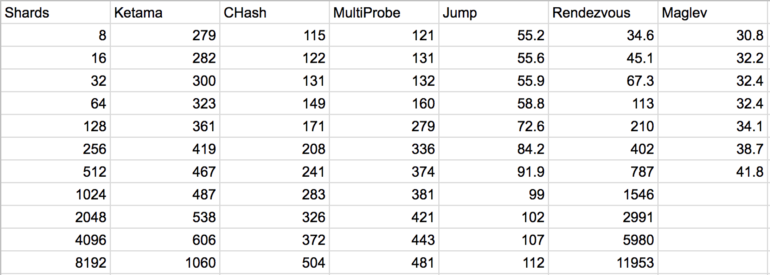
\includegraphics[width=14cm]{consistent-hashing-benchmarks.png}
    \end{figure}
    
    \subsubsection{Probabilistic Data Structures}
    A \textbf{Bloom filter} is a data structure designed to tell you, rapidly and memory-efficiently, whether an element is present in a set. The price paid for this efficiency is that a Bloom filter is a probabilistic data structure: it tells us that the element either definitely is not in the set or may be in the set, i.e. it has false positives but never false negatives. Because of this, it is commonly used for deduplication, for example when adding a job into a pool.
    
    To briefly explain how bloom filter works, an empty bloom filter is a bit array of m bits (all 0). There are also $k$ hash functions that map each element to one of the m bits. So when we add a new element into the bloom filter, we will get $k$ bits from the hash functions and set all of them to 1. Thus, when we check the existence of an element, we first get the $k$ bits for it and if any of them is not 1, we know immediately that the element doesn't exist. However, if all of the $k$ bits are 1, this can come from the combination of several other elements.
    
    
    The \textbf{count–min sketch} (CM sketch) is a probabilistic data structure that serves as a frequency table of events in a stream of data. It uses hash functions to map events to frequencies, but unlike a hash table uses only sub-linear space, at the expense of overcounting some events due to collisions.
    
    \subsubsection{Design Patterns and OOP}
    See OOP and Design Patterns notebook\footnote{https://github.com/lukepereira/notebooks}
    
    \subsubsection{Protocol Buffers}
    Protocol buffers are a data storage and exchange format, notably used for RPC - communication between programs or computers.
    
    Alternatives include language-specific serialization (Java serialization, Python pickles, etc.), tabular formats like CSV and TSV, structured text formats like XML and JSON, and other binary formats like Apache Thrift. Conceptually these are all just different ways of representing structured data, but in practice they have different pros and cons.

    
    \subsubsection{Logs}
    An append-only file for storing data. A write-ahead log is used to make a storage engine resilient against crashes, a log structured storage engine uses logs as its primary storage format, a replication log is used to copy writes from a leader to followers, and an event log can represent a data stream.
    
    Metrics should be used alongside logs for more accurate analysis of system behaviours.

    \subsubsection{Multitier Architecture}
     Multilayered architecture is a client–server architecture in which presentation, application processing and data management functions are physically separated. 
    
    The most widespread use of multitier architecture is the three-tier architecture.

    \begin{enumerate}[i.]
        \item \textbf{Presentation tier} -- In simple terms, it is a layer which users can access directly (such as a web page, or an operating system's GUI).
        \item \textbf{Application tier} -- The logical tier (a.k.a business logic, logic tier, or middle tier) is pulled out from the presentation tier and, as its own layer, it controls an application’s functionality by performing detailed processing.
        \item \textbf{Data tier} -- The data tier includes the database servers, file shares, etc. and the data access layer that encapsulates those persistence mechanisms. The data access layer should provide an API to expose the data to the application tier for providing methods of managing the stored data without exposing or creating dependencies on the data storage mechanisms.
    \end{enumerate}
    
    \subsubsection{Services}
    ``Service” here means a distributed system that incorporates higher-level logic than a storage system and typically has a request-response style API. Be on the lookout for code changes that would be easier to do if the code existed in a separate service instead of in your system.
    
    An extracted service provides the benefits of encapsulation typically associated with creating libraries. However, extracting out a service improves on creating libraries by allowing for changes to be deployed faster and easier than upgrading the libraries in its client systems.
    
    The coordination costs of using a service is also much lower than a shared library when there are multiple client systems. Upgrading a library, even with no API changes needed, requires coordinating deploys of each client system.

    \subsubsection{Back of the Envelope Calculations}
    Ability to estimate performance of a system design without actually having to build it is an important skill.
    
    Given a basic problem definition, how do you choose the "best" solution? Best could be simplest, highest performance, easiest to extend, etc.
    
    \textbf{Numbers Everyone Should Know (2012)}
    \begin{table}[H]
    \begin{tabular}{|l|l|}
    \hline
        L1 cache reference & 0.5 ns  \\
        Branch mispredict &  5 ns \\
        L2 cache reference & 7 ns \\
        Mutex lock/unlock & 25 ns \\
        Main memory reference & 100 ns \\
        Compress 1K bytes with Zippy & 3,000 ns \\
        Send 2K bytes over 1 Gbps network & 20,000 ns \\
        Read 1 MB sequentially from memory & 250,000 ns \\
        Round trip within same datacenter & 500,000 ns \\
        Disk seek & 10,000,000 ns \\
        Read 1 MB sequentially from disk & 20,000,000 ns \\
        Send packet CA $\to$ Netherlands $\to$ CA & 150,000,000 ns \\
    \hline
    \end{tabular}
    \end{table}
    
    \textbf{How many operations in one second? (2020)}
    \begin{table}[H]
    \begin{tabular}{|l|l|l|}
    \hline
        C  & iterations over for loop & 550,000,000 \\
        python & iterations over for loop & 68,000,000 \\
        python & insertions into a dictionary & 11,000,000 \\
        python & HTTP requests parsed in one second & 25,000 \\
        python & download google webpage & 4 \\
        python & start the python interpreter (-c python) & 77 \\
        python & bytes written to output file  &  342,000,000 \\
        python & bytes written to memory & 2,000,000,000 \\
        bash & bytes searched (grep)  &  2,000,000,000 \\
        bash & files searched (find) & 325,000 \\
        python & parse messages of size 64k encoded via JSON &  449 \\
        python & parse messages of size 64k encoded via msgpck &  4,000 \\
         python & select a row from an indexed SQLite table with 10M rows &  53,000 \\
        python & select a row from an unindexed SQLite table with 10M rows &  2 \\
        python & bytes hashed using md5sum &  455,000,000 \\
        python & bytes hashed using bcrypt & 3 \\
        C & size of array allocated and filled in order & 376,000,000 \\
        C & size of array allocated and filled out of order & 68,000,000 \\
    \hline
    \end{tabular}
    \end{table}
    
    
    Example: How long will it take to generate image results page (30 thumbnails)?
    
    Design 1: Read serially, thumbnail 256K images on the fly $\implies$  \newline
    30 seeks * 10 ms/seek + 30 * 256K / 30 MB/s = 560 ms
    
    Design 2: Issue reads in parallel: $\implies$ \newline 10 ms/seek + 256K read / 30 MB/s = 18 ms (Ignores variance, so really more like 30-60 ms, probably)
    
    \textbf{Throughput} is defined as the number of jobs processed over a given interval of time, transactions per second (TPS) measures the number of atomic actions. Each incoming transaction will have some level of operations it triggers where the number of CPU instructions entails \textbf{work done per transaction}. A user often waits or processes responses before submitting again. This delay is the user \textbf{think time} that falls between requests and can be taken into account when calculating optimum system load and incoming request distributions.
    
    \subsubsection{Canary Deployments}
    In software testing, a canary is a push of programming code changes to a small group of end users who are unaware that they are receiving new code. Because the canary is only distributed to a small number of users, its impact is relatively small and changes can be reversed quickly should the new code prove to be buggy. Canary tests, which are often automated, are run after testing in a sandbox environment has been completed.
    
    \subsubsection{Feature Flags}
    Feature flags are a common way product engineers roll out new features in a system. Feature flags are typically associated with frontend A/B testing where they are used to show a new design or feature to only some of the userbase. But they are a powerful way of replacing infrastructure as well.
    
    Using a feature flag, you can slowly ramp up writes to the new service in parallel to the writes to the old service to make sure its write path is correct and fast enough. After the write path is at 100\% and backfilling into the service’s datastore is complete, you can use a separate feature flag to start reading from the service, without using the data in user responses, to check for performance problems. Another feature flag can be used to perform comparison checks on read of the data from the old system and the new one. And one final flag can be used to slowly ramp up the ``real” reads from the new system.

    The use of feature flags means accepting that having multiple versions of infrastructure and data is a norm, not an rarity. Feature flags are best understood as a trade-off, trading local complexity (in the code, in one system) for global simplicity and resilience. 
    
\newpage
\section{Networks}
    \subsection{Concepts}
    
    \subsubsection{Caching}
    A cache is a component that remembers recently used data in order to speed up future reads of the same data. It is generally not complete: thus, if some data is missing from the cache, it has to be fetched from some underlying, slower data storage system that has a complete copy of the data.
    
    Cached data must be relatively small since cached data is generally stored in memory.
    
    CPUs these days have L1 and L2 caches, which are much faster to access than main memory. This means that accessing memory sequentially (where the CPU can load a bunch of data into a cache) will normally give you faster code than accessing memory out of order.
    
    In an \textbf{in-process cache}, your cache elements are local to a single instance of your application. 
    
    In a \textbf{distributed cache}, each object is replicated among multiple independent machines, multiple cache nodes.
    
    \textbf{Memcached} is a commonly used distributed memory-caching system. It caches data and objects in RAM to reduce the number of times an external data source (such as a database or API) must be read.
    
    \textbf{Cache coherence} is the uniformity of shared resource data that ends up stored in multiple local caches. When clients in a system maintain caches of a common memory resource, problems may arise with incoherent or inconsistent data.
    
    The common solution to concurrency issues is using a lock, but has the downside of greatly affecting performance. An alternative is to use commit logs: we can store all the mutations to the cache into log files rather than update immediately, then a background processes will execute all the logs asynchronously. Writing cached data back to persistent storage is bad. A common presentation of this flaw is user information mysteriously reverting to a previous value. 
    
    A \textbf{cache eviction policy} or cache replacement algorithm is a way of deciding which element to evict when the cache is full. Some popular policies include:
    \begin{enumerate}
        \item First-in first-out (FIFO)
        \item Last-in first-out (LIFO)
        \item Least recently used (LRU)
        \item  Random Replacement (RR) -- As the term suggests, we can just randomly delete an entry.
        \item Least frequently used (LFU) -- We keep the count of how frequent each item is requested and delete the one least frequently used.
        \item W-TinyLFU -- A modern eviction policy that resolves the problem of LFU storing an item that was used frequently in the past, but is no longer used. W-TinyLFU solves this problem by calculating frequency within a time window. It also has various optimizations of storage.
    \end{enumerate}
    
    \subsubsection{LRU Cache}
    The way LRU cache works is quite simple. When the client requests resource A, it happens as follow:
    
    \begin{enumerate}
        \item If A exists in the cache, we just return immediately.
        \item If not and the cache has extra storage slots, we fetch resource A and return to the client. In addition, insert A into the cache.
        \item  If the cache is full, we kick out the resource that is least recently used and replace it with resource A.
    \end{enumerate}
    
    An LRU cache should support the operations: lookup, insert and delete. We may use two data structures to implement an LRU Cache.
    \begin{enumerate}
        \item Queue which is implemented using a doubly linked list. The queue is useful for maintaining ordering while the linked list will optimize for insertions and deletions.
        
        The maximum size of the queue will be equal to the total number of frames available (cache size). The most recently used pages will be near front end and least recently pages will be near the rear end.
        
        \item A Hash with page number as key and address of the corresponding queue node as value. This allows $\mathcal O(1)$ lookups.
    \end{enumerate}
    
    

    For example, to combine all these operations we can use queue implemented by a doubly linked list to store all the resources. Also, a hash table with resource identifier as key and address of the corresponding queue node as value is needed.
    
    \begin{enumerate}
        \item When resource A is requested, we check the hash table to see if A exists in the cache.
        \item If exists, we can immediately locate the corresponding queue node and return the resource. If not, we’ll add A into the cache.
        \item If there is enough space in the cache, we may add A to the end of the queue and update the hash table. Otherwise, we need to delete the least recently used entry by removing the head of the queue and the corresponding entry from the hash table.
    \end{enumerate}  
    
    \subsubsection{Request Protocols}
    \textbf{HTTP/2} leaves all of HTTP 1.1's high-level semantics, such as methods, status codes, header fields, and URIs, the same but has some speed improvements over HTTP, i.e. multiple requests on single connection, multiplexing requests and responses to avoid blocking requests, header compression, and prioritization of requests.
    
    \textbf{Websockets} provide bi-direction communication between client and server.
    
    Bidirectional-streams Over Synchronous HTTP (\textbf{BOSH}) is a transport protocol that emulates a bidirectional stream between two entities (such as a client and a server) by using multiple synchronous HTTP request/response pairs without requiring the use of polling or asynchronous chunking.
    
    With \textbf{long polling}, a client requests information from the server exactly as in normal polling, but with the expectation the server may not respond immediately. If the server has no new information for the client when the poll is received, instead of sending an empty response, the server holds the request open and waits for response information to become available.
    
    \subsubsection{TCP and UDP}
    Transmission Control Protocol (TCP) is a connection-oriented protocol, whereas User Datagram Protocol (UDP) is a connectionless protocol. The speed for TCP is slower than UDP. However, TCP does error checking and also makes error recovery  while UDP performs error checking but it discards erroneous packets.
    
    \subsubsection{IPv4 and IPV6}
    IPv4 is a 32-Bit IP Address: numeric address, and its binary bits are separated by a dot.
    
    IPv6 is 128 Bit IP Address: alphanumeric address whose binary bits are separated by a colon.

    \subsubsection{DNS Lookup}
    A domain name server (DNS) does translation of IP to readable domain name
    
    \subsubsection{HTTPS and TLS}
    Transport Layer Security adds security via a signed certificates to HTTP
    
    A public key infrastructure manages and stores public keys. A certificate authority tells us if public key is from correct identity and prevents MITTM attacks.

    \subsubsection{Symmetric and Asymetric Encryption}
    Symmetric encryption uses a single key that needs to be shared among the people who need to receive the message. AES is symmetric.
    
    Asymmetrical encryption uses a pair of public key and a private key to encrypt and decrypt messages when communicating. RSA is asymmetric.
    
    Asymmetric encryption is more expensive, should be used for smaller amounts of data
    
    \subsubsection{Internet Protocol Suite and OSI}
    
    The Internet protocol suite predates the OSI model, which a more comprehensive reference framework for general networking systems. The model partitions a communication system into the following abstraction layers:
    \begin{enumerate}[i.]
        \item The \textbf{application layer} is the scope within which applications, or processes, create user data and communicate this data to other applications on another or the same host.
        \item The \textbf{transport layer} performs host-to-host communications on either the local network or remote networks separated by routers.
        \item The \textbf{internet layer} exchanges datagrams across network boundaries. It provides a uniform networking interface that hides the actual topology (layout) of the underlying network connections.
        \item The \textbf{link layer} defines the networking methods within the scope of the local network link on which hosts communicate without intervening routers.
    \end{enumerate}
    
    The Open Systems Interconnection model (OSI model) is a conceptual model that characterises and standardises the communication functions of a telecommunication or computing system. The model partitions a communication system into the following abstraction layers:

    \begin{multicols}{2}
    \begin{enumerate}[i.]
        \item \textbf{Physical Layer}
        \item \textbf{Data Link Layer}
        \item \textbf{Network Layer}
        \item \textbf{Transport Layer}
        \item \textbf{Session Layer}
        \item \textbf{Presentation Layer}
        \item \textbf{Application Layer}
    \end{enumerate}
    \end{multicols}
    
    \subsubsection{L4 and L7 Load Balancers}
    A load balancer receives requests and delegates them to servers according to some policy, i.e. round robin, load average.
    
    Layer4 (L4) works on Layer4 (and Layer3) of the OSI model. When a client makes a request, it creates a TCP connection with the load balancer. The Load Balancer then uses the same TCP connection that the client created with it, to connect with one of the upstream servers. The source and destination IP of each packet is changed by the load balancer using NAT (Network address translation). When a response is received from the server, the same translation is performed again at the load balancer.
    
    There is another type of L4 load balancer known as TCP/UDP termination load balancers where there are two different TCP connections. When using L4 load balancers, we are unaware of the data. This means we cannot make any decisions based on data in our request. The only thing we have is IPs (source and destination)and ports. Load balancer can work at TCP level as long as it is at layer4. This is because TCP load balancers are for applications that do not use HTTP. Layer7 in the OSI model, for example, expects all network traffic to be HTTP.
    
    Cons: No smart load balancing, Doesn’t work with streaming/keep-alive connections, No TLS termination

    Layer7 (L7) works on Layer7 (Layer6 and Layer5) of the OSI model. When a client makes a request, it creates a TCP connection with the load balancer. The Load Balancer then creates a new TCP connection with one of the upstream servers. Thus, there are 2 TCP connections as compared to 1 in a TCP/UDP passthrough L4 Load balancer.
    
    Since we are at layer7, we are aware of the data in our request. This allows us to perform a variety of operations like: Authentication, Smart Routing, TLS termination
    
    L7 load balancer creates a TCP connection with every upstream for a single client connection rather than choosing a single upstream. This means when A creates a connection with the load balancer, the load balancer creates two connections one with C and one with D.
    
    \subsubsection{CDN and Edge Computing}
    Content Delivery Networks (CDN) serve static content with low-latency and low-cost using servers closest to the client. On the other hand, object storage is durable and highly available and is typically used as a reliable back-up of the content in a CDN.
    
    Edge computing performs computation or processing using servers closest to the client.
    
    \subsubsection{Locality}
    A performance optimization: putting several pieces of data in the same place if they are frequently needed at the same time.
    
    The closer the processing and caching of your data is kept to its persistent storage, the more efficient your processing, and the easier it will be to keep your caching consistent and fast. Networks have more failures and more latency than pointer dereferences and reads.
    
    Of course, data-locality means being nearby in space, but it also means nearby in time. If multiple users are making the same expensive request at nearly the same time, perhaps their requests can be joined into one. If multiple instances of requests for the same kind of data are made near to one another, they could be joined into one larger request. Doing so often affords lower communication overheard and easier fault management.
    
    \subsubsection{Percentiles}
    A way of measuring the distribution of values by counting how many values are above or below some threshold. For example, the 95th percentile response time during some period is the time t such that 95\% of requests in that period complete in less than t, and 5\% take longer than t.
    
    Percentiles (50th, 99th, 99.9th, 99.99th) are more accurate and informative than averages in the vast majority of distributed systems. Using a mean assumes that the metric under evaluation follows a bell curve but, in practice, this describes very few metrics an engineer cares about. If the metric doesn’t follow a bell curve, the average is meaningless and leads to incorrect decisions and understanding. Avoid the trap by talking in percentiles. Default to percentiles, and you’ll better understand how users really see your system.
    
    \subsubsection{Metrics}
    Exposing metrics (such as latency percentiles, increasing counters on certain actions, rates of change) is the only way to cross the gap from what you believe your system does in production and what it actually is doing. 
    
    Log files are good to have, but they tend to mislead. For example, it’s very common for the logging of a few error classes to take up a large proportion of a space in a log file but, in actuality, occur in a very low proportion of requests. Outages are often extended by engineers over-emphasizing something odd seen in the log without first checking it against the metrics.
    
    % \subsubsection{Synchronous and Asynchronous}
    
    \subsubsection{Backpressure}
    Forcing the sender of some data to slow down because the recipient cannot keep up with it. Also known as flow control.
    
    Backpressure is the signaling of failure from a serving system to the requesting system and how the requesting system handles those failures to prevent overloading itself and the serving system. Designing for backpressure means bounding resource use during times of overload and times of system failure. This is one of the basic building blocks of creating a robust distributed system.
    
    Implementations of backpressure usually involve either dropping new messages on the floor, or shipping errors back to users (and incrementing a metric in both cases) when a resource becomes limited or failures occur. Timeouts and exponential back-offs on connections and requests to other systems are also essential.

    Without backpressure mechanisms in place, cascading failure or unintentional message loss become likely. When a system is not able to handle the failures of another, it tends to emit failures to another system that depends on it.
    
    \subsubsection{The Two Generals and Byzantine Generals Problem}
    The Two Generals' Problem is a thought experiment in which two generals are only able to communicate with one another by sending a messenger through enemy territory. The experiment asks how they might reach an agreement on the time to launch an attack, while knowing that any messenger they send could be captured. It is meant to illustrate the pitfalls and design challenges of attempting to coordinate an action by communicating over an unreliable link.
    
    It relates to Transmission Control Protocol, where it shows that TCP can't guarantee state consistency between endpoints.

\newpage
\section{System Design Interview}
\subsection{Outline}
\begin{enumerate}
    \item Requirements - 5-10 mins
    \begin{enumerate}
        \item Exploratory Questions
        \item Use Cases
        \item Functional/Out of scope/Extended
        \item Non-Functional
    \end{enumerate}
    \item Capacity Estimates - 2-5 mins
    \item High Level Design - 5-10 mins
    \item Data Model / APIs - 5 mins
    \item Scale each component in HLD depending on NFR - 10 mins
    \item Verify your design / Discuss trade-offs - 5 mins
\end{enumerate}

\subsection{Process}

\subsection{Architectural Patterns}
    
    A \textbf{real-time messaging} server connects clients to a simulated thread and assigns them a receiving queue with an id or reference being stored into a table. When sending messages to another client, the service checks for a receiver in the queue reference table: if the recipient has a queue assigned to them , then they currently connected, so the message is pushed to the receiver's queue and read by their client. Otherwise the message is written to a persistent database. Upon reconnecting, the client polls the persistent database for any unread messages and updates their state and returns the message to the client.

    \textbf{Timelines and news feeds} constructed by user follows or subscribes, like in Twitter, cannot make multiple queries to a database for all follower ids then each of their recent tweets on every visit to the homepage. Instead a distributed cache like Redis pre-computes and stores relevant posts from people the user follows in a data structure like a list. When a user makes a post, the content is distributed to all of their followers. If posting user's follower count is above some threshold, we don't distribute their posts to other users but store in their own cached list and we add the user to a table of users with high-follower counts. When fetching a timeline, the service retrieves messages already pre-loaded in their queue from accounts with low/medium follower and then polls the cached data of any other high-follower users, then collates all the data into a feed based on timestamps and other rating rules.
    
    \textbf{Trending analysis} may use a streaming service like Kafka to run data through a pipeline made of stateless operators that can be scaled and run in parallel with outputs connected to one another by queues, i.e. filter, parse, geolocation, count location, count tags, rank.
    
    \textbf{Real-time ranking and leader boards} would not be able to scale when using traditional RDBMS. Instead we can use the ordered sets data structure offered by Redis, an in-memory distributed cache. Sorted sets contain a list of members with associated scores. Although set members are unique, score values are permitted to repeat. Scores are used to rank the list in ascending order. One key difference between sorted sets and relational databases is when the tool sorts the list. During insert or update operations, sorted sets automatically position the item in the right order. Because of this pre-sorting, queries run significantly faster. You can quickly and efficiently query the middle of the list or get the rank of a specific member. Sorted sets finds specific rankings in logarithmic time proportional to the number of members. By contrast, relational databases order items during querying, adding computational burden to the database. Obtaining the rank of a specific player involves quadratic time complexity.
    
    \textbf{A distributed log system} can use an ELK stack. LogStash or Filebeat can be used for ingesting logs from various sources by running as a daemon directly on servers and configured to read and parse data from desired log files. It can write to an Elasticsearch cluster which can be queried by date ranges or keywords using Kibana.
    
    A \textbf{cloud-based file storage system} like google drive or dropbox usually provides fast uploads and versioning. Instead of storing the full copies of each modified version in cloud storage and to increase upload speeds, we can split up files into chunks that will each be assigned a hash. The chunks are all uploaded concurrently and the chunk hashes, their orders and other details are captured in metadata files that are stored both internally and in an external SQL db. When a file is modified, only the chunk containing changes will be uploaded and have a its new hash updated. To manage synchronization among all of a client's devices, a queue is maintained on the server that updates the local state of any client as they connect to the service. If we can't use a managed cloud storage system like s3, we can distribute files among different hard-drive heavy servers with replicas, and use a metadata db to store mappings of files to servers that can also maintain health and fail overs of the storage servers.
    
    Sharing multimedia files are handled by first uploading to a cloud storage system and CDN and then returning a hash of the file's location. The hash is then shared to the recipient at the app level that uses it to retrieve and download the original multimedia file. Metadata of the file is stored in a standard SQL database.
    
    A \textbf{real-time map}, like in a video game, requires low latency between user action and feedback between many users. To achieve this, a client interacts with 3 services: a connection server, a world server and a game server. The connection/proxy server handles overhead of connection auth/decoding/decryption/decompression request. The world server assigns a client to a game server depending on their location in the map, tracks the players state in order to orchestrate region assignments, and coordinates the different game servers to achieve any global game logic. Multiple game servers exist for different pieces of the map and they run the actual game sessions. Less popular locations in the map can be assigned to a single server. Each region session is a singleton. To handle crossing regions seamlessly, adjacent game servers share information about state of objects and players who are near edges directly with each other. When working with real world data or large maps, it can be expensive to use longitude and latitude, instead our regions can be given rectangular or Spherical Geometry (google's s2) with ids.
    
    A \textbf{real-time tracking and dispatch system} like Uber divides global map into cells using spherical geometry based cells, uses consistent hashing to distribute cell data to servers. A client's finds all cells it nearby radius intersects. Web-sockets listen to streaming data from user and driver clients. Pipeline gets available drivers from client web-socket connections, appending streaming jobs into Kafka queue and determines appropriate region id. User requests are sent to dispatch API which assigns jobs to appropriate regional server and determines ETA using 3rd party maps API (Google, Mapbox). Adjacent regional servers communicate with each other to reach consensus on which drivers to notify.
    
    Generating unique hashes in a distributed system can use a standalone \textbf{Key Generation Service} (KGS) that generates random six-letter strings beforehand and stores them in a database (key-DB). This prevents waiting for the computation and avoids duplication or collisions. To avoid concurrency issues, the KGS can use two tables to store keys: one for keys that are not used yet, and one for all the used keys. As soon as KGS gives keys to one of the servers, it can move them to the used keys table. KGS can always keep some keys in memory so that it can quickly provide them whenever a server needs them. KGS also has to make sure not to give the same key to multiple servers. For that, it must synchronize (or get a lock on) the data structure holding the keys before removing keys from it and giving them to a server. To prevent the KGS from being a single point of failure, we can have a standby replica of KGS that can take over to generate and provide keys.
    
    \textbf{Document search engine} make use of offline pipeline to pre-processes document: filters out unnecessary stop words noise, uses stemming or lemmatisation to get common base words, converts to lowercase. Then inserts word into an inverted index with rows of keywords, frequency, document id with occurrence. Rankings can be derived using page rank with other features like freq, reputation and age of the page. Take into account conjunctive (AND) or disjunctive (OR) on key words, order of key words. Keywords are sorted alphabetically allowing for binary search on prefixes or use Tries/suffix trees. Searching across several disparate data centers can be done using a scatter and gather approach, where a service queries several DBs in parallel then collates their results. If a server is taking too long, instead of waiting we can return partial results.
    
    In a \textbf{video streaming service}, a load balancer routes client to different servers. Pre-processing pipeline transcodes video into different format/codecs/resolutions and creates multiple copies of video for different devices and internet speeds. This can be done offline by chunking, transcoding, and merging the large files and then uploading to distributed CDN network.
    
    \textbf{Collaborative documents} use operation transformation event parsing and differential sync. OT is an optimistic concurrency mechanism that allows two editors to modify the same document that simplifies resolving conflicts so that neither user resolution nor locking is necessary. We have an authoritative server that receives all operations from users and serves unified the document. It works by storing a chronological list for each document of every change. ``Type an H at position 0". ``Type a i at position 1". If users are collaboratively editing, we get concurrent edits, then the first edit to arrive at the server gets recorded as usual. If the second edit is out of date, we use the log of operations as a reference to figure out what the user really intended, usually this just means updating character positions. Then we pretend as if that's what the user meant all along and append the new (edited) operation. Its like real-time git-rebase. Let a = client operation, b = server operation, a' = server operation, b' = client operation. Then, operational transformations can be expressed xform(a,b) = (a',b'), where b' composed a = a' composed b. Differential synchronization works similarly to git diff by detecting differences in a client's local copy vs. a global copy which is stored and updated as a patch on both the local and remote copies. The server copy of the document is the source of truth, it broadcasts the changed copy to all connected clients and updates their local copy. To save space, only the diff is saved instead of the complete redundant parts of the document. 
    
    The big problem with OT is that dependency on a centralized server. \textbf{Conflict-free Replicated Data Type} (CRDTs) approach the problem slightly differently to allow real-time editing without needing a central source of truth. they provide Strong Eventual Consistency (SEC), i.e. all actors will eventually converge to the same state without data loss.
    
    In a \textbf{web crawler}, seed URLs are generated from script and stored in database or file with a null last visited date. A management service periodically reads from the database, performs HTTP head requests to detect updates and inserts URL with metadata into pipeline of priority queues. A server using curl/headless browser/server-side rendering waits for free threads to read from the queue and then fetches and renders web-pages asynchronously. To cut down the request time, we can use our own DNS resolver to get the host IP of the websites before fetching them. After rendering web-page, we can cache in local memory or in a distributed cache like Redis for upcoming server processing and can store a Simhash hash of the core page content in a database to compare diffs and avoid reprocessing unchanged pages. The web-page is added into a queue for further page analysis/processing like extracting more unique URLs on the domains or desired content. Visited URLs are upserted into the URLs database with the current time and any unique URLs are passed back into the management service queues to continue exploration of the web domain.
    
    To handle \textbf{distributed transactions in micro-services}, we can use sagas or two/three-phase commits. Two-phase commit consists of two parts: prepare and commit. The orchestrator receives a client request for a transaction and forwards it two a coordinator to create a transaction id and prepares a transaction by performing any prerequisite actions to micro-services with timeout detection. If they are successful, then the coordinator commits and performs the final action, otherwise it rolls-back previous actions and returns a failure error code.
    
    A \textbf{job scheduler} can use an SQL database with an indexed date-time column and status column as a priority queue to enque process and deque jobs while remaining consistent.


\newpage
\begin{thebibliography}{}
\bibitem{a}
Kleppmann, M. (2017). Designing Data-Intensive Applications. Beijing: O'Reilly. ISBN: 978-1-4493-7332-0

\bibitem{b}
https://www.somethingsimilar.com/2013/01/14/notes-on-distributed-systems-for-young-bloods/

\bibitem{c}
https://codahale.com/you-cant-sacrifice-partition-tolerance/


\bibitem{d}
https://research.cs.cornell.edu/ladis2009/talks/dean-keynote-ladis2009.pdf

\bibitem{e}
http://computers-are-fast.github.io/

\bibitem{f}
https://medium.com/@dgryski/consistent-hashing-algorithmic-tradeoffs-ef6b8e2fcae8

\end{thebibliography}
\end{document}
